\section{Clustering}

\subsection{K-means Clustering (14 points)}

\begin{enumerate}

\item \textbf{(6 Points)}
Given $n$ observations $X_1^n = \{X_1, \dots, X_n\}$, $X_i \in \Xcal$, the K-means objective
is to find $k$
($<n$) centres $\mu_1^k = \{\mu_1, \dots, \mu_k\}$, and a rule $f:\Xcal \rightarrow
\{1,\dots, K\}$ so as to minimize the objective

\begin{equation}
J(\mu_1^K, f; X_1^n) = \sum_{i=1}^n \sum_{k=1}^K \indfone(f(X_i) = k) \|X_i - \mu_k\|^2
\label{eqn:kmeans}
\end{equation}

Let $\Jcal_K(X_1^n) = \min_{\mu_1^k, f} J(\mu_1^K, f; X_1^n)$. Prove that
$\Jcal_{K}(X_1^n)$ is a non-increasing function of $K$.

\begin{soln}
Lets begin by finding what $f,\mu_K$ are. Although we cannot find the best $\mu$ and $f$ at the same time, we can:
\begin{itemize}
    \item fix $\mu$, we find the best $f$ exactly. Also called the Assignment Step.
    \begin{align*}
        \Jcal_K(X_1^n) &= \min_{f} J(\mu_1^K, f; X_1^n)\\
        &= \min_{f} \sum_{i=1}^n \sum_{k=1}^K \indfone(f(X_i) = k) \|X_i - \mu_k\|^2 \\
        &= \min_{f} \sum_{k=1}^K \indfone(f(X_1) = k) \|X_1 - \mu_k\|^2 + \ldots + \sum_{k=1}^K \indfone(f(X_n) = k) \|X_n - \mu_k\|^2
    \end{align*}
    Thus we can minimize each of the above term individually by setting
    $$
        f(X_i) = \argmin_{k} \|X_i - \mu_k\|^2
    $$
    \textbf{Which means to assign the point to the cluster whose centroid is closest.}
    \item fix $f$, we find the best $\mu$ exactly. Also called the Update Step.
    \begin{align*}
        \Jcal_K(X_1^n) &= \min_{\mu_1^K} J(\mu_1^K, f; X_1^n)\\
        &= \min_{\mu_1^K} \sum_{i=1}^n \sum_{k=1}^K \indfone(f(X_i) = k) \|X_i - \mu_k\|^2 \\
        &= \min_{\mu_1^K} \sum_{i=1}^n \indfone(f(X_i) = 1) \|X_i - \mu_1\|^2 + \ldots + \sum_{i=1}^n \indfone(f(X_i) = K) \|X_i - \mu_K\|^2
    \end{align*}
    The individual terms can be minimized by setting:
    $$
        \mu_k = \argmin_{\mu} \sum_{i=1}^n\indfone(f(X_i) = k)\|X_i - \mu\|^2 = \frac{\sum_{i=1}^n\indfone(f(X_i) = k)X_i}{\sum_{i=1}^n\indfone(f(X_i) = k)}
    $$
    \textbf{Thus pick a centroid of a cluster as the mean of all points in that cluster.}
\end{itemize}

Now lets pick a setting where we increase the number of clusters by 1 i.e. total clusters are $\mathbf{K+1}$. \\
Let $f^{K}(X_i)$ assign the cluster to a point in a setting with K cliusters.
    
\begin{itemize}
    \item Assignment Step proof: 
    
    A point will be assigned to this new cluster if and only if its closer to the center of this new cluster
    $$
        \|X_i - \mu_{K+1}\|^2 < \|X_i - \mu_{k}\|^2 \;\forall\;k=1,2,...,K
    $$ 
    Thus decreasing the total objective value than before. The worst case scenario is when no point is assigned to this new cluster in which case the objective value remains the same.\\
    
    \textbf{Hence proved the objective value can never increase during assignment step when increasing $K$.}

    \item Update Step proof:
    If a point is assigned from cluster $k$ to $K+1$. 
    \begin{itemize}
        \item Let the cluster $k$ with less points be called $k'$. \\
        The new $\mu_{k'}$ will change from before if and only if it decreases the total objective value of leftover points in its cluster. If the new $\mu_{k'}$ increases the total objective value then it was better off staying at $\mu_k$.
        $$
            \sum_{i=1}^n\indfone(f^{K+1}(X_i) = k')\|X_i - \mu_{k'}\|^2 \leq \sum_{i=1}^n\indfone(f^{K+1}(X_i) = k')\|X_i - \mu_{k}\|^2
        $$
        \item As for the point assigned to $K+1$.\\
        % We can easily say $\|X_i - \mu_{k}\|^2 \leq \|X_i - \mu_{k'}\|^2$, otherwise $\mu_{k'}$ would have been the original centroid for cluster $k$ as it reduces the distance of all points in the original cluster.\\
        Now if the sum of objective value in the original setting is less than in the current one i.e.:
        $$
            \sum_{i=1}^n\indfone(f^{K+1}(X_i) = K+1)\|X_i - \mu_{f^{K}(X_i)}\|^2 \leq \sum_{i=1}^n\indfone(f^{K+1}(X_i) = K+1)\|X_i - \mu_{K+1}\|^2
        $$
        Where $\mu_{f^{K}(X_i)}$ is the centroid of their cluster in the original setting with only K cluster \\
        Then:
        $$
            \mu = \frac{\sum_{i=1}^n\indfone(f^{K+1}(X_i) = K+1)\mu_{f^{K}(X_i)}}{\sum_{i=1}^n\indfone(f^{K+1}(X_i) = K+1)}
        $$
        gives equal objective value as the original setting and is a better choice of $\mu_{K+1}$. Thus the sum of objective values for newly assigned points can also never increase.
    \end{itemize}
    \textbf{Thus increasing $K$ will increase the total objective value for neither the set of points that don't change cluster nor those which do during the Update Step.}
\end{itemize}
\end{soln}

\item \textbf{(8 Points)}
Consider the K-means (Lloyd's) clustering algorithm we studied in class. We
terminate the algorithm when there are no changes to the objective.
Show that the algorithm terminates in a finite number of steps.

\begin{soln}
    We can see above that the K-mean algorithm moves in a fashion to reduce the objective $\Jcal_K(X_1^n) = \min_{\mu_1^k, f} J(\mu_1^K, f; X_1^n)$. Now for \textbf{fixed set of points} $X_1^n = \{X_1, \dots, X_n\}$, $X_i \in \Xcal$ and a \textbf{fixed $K$} there can only be a finite set of assignments of points to the clusters i.e. only a \textbf{finite number of objective values} and even if the algorithm iterates over all of them it will eventually choose the one with minimum objective value $\Jcal_K(X_1^n)$ and terminate after those finite set of iterations and converge to a solution. 
\end{soln}

\end{enumerate}



\subsection{Experiment (20 Points)}

In this question, we will evaluate
K-means clustering and GMM on a simple 2 dimensional problem.
First, create a two-dimensional synthetic dataset of 300 points by sampling 100 points each from the
three Gaussian distributions shown below:
\[
P_a = \Ncal\left(
\begin{bmatrix}
-1 \\ -1
\end{bmatrix},
\;
\sigma\begin{bmatrix}
2, &0.5 \\ 0.5, &1
\end{bmatrix}
\right),
\quad
P_b = \Ncal\left(
\begin{bmatrix}
1 \\ -1
\end{bmatrix},
\;
 \sigma\begin{bmatrix}
1, &-0.5 \\ -0.5, &2
\end{bmatrix}
\right),
\quad
P_c = \Ncal\left(
\begin{bmatrix}
0 \\ 1
\end{bmatrix},
\;
 \sigma\begin{bmatrix}
1 &0 \\ 0, &2
\end{bmatrix}
\right)
\]
Here, $\sigma$ is a parameter we will change to produce different datasets.

\begin{soln}
    \begin{figure}[H]
        \begin{subfigure}{0.5\textwidth}
            \centering
            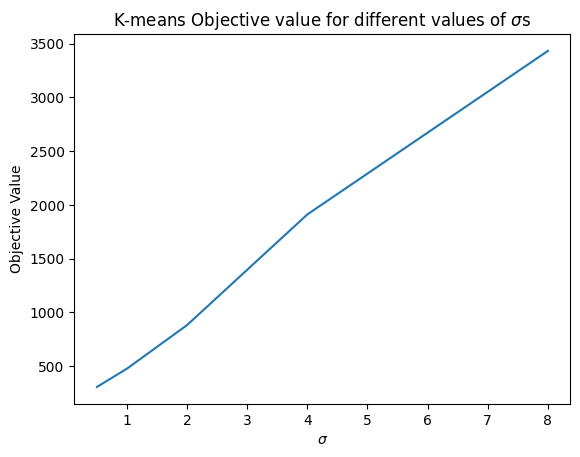
\includegraphics[scale=0.35]{Images/q12/q12_km.png}
        \end{subfigure}%
        \begin{subfigure}{0.5\textwidth}
            \centering
            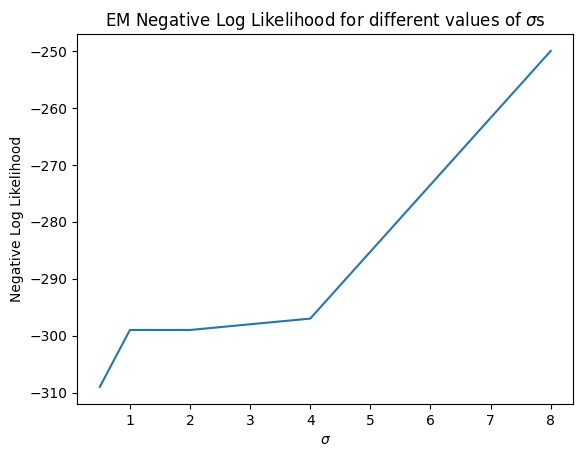
\includegraphics[scale=0.35]{Images/q12/q12_em.png}
        \end{subfigure}
    \end{figure}
    \begin{figure}[H]
        \centering
        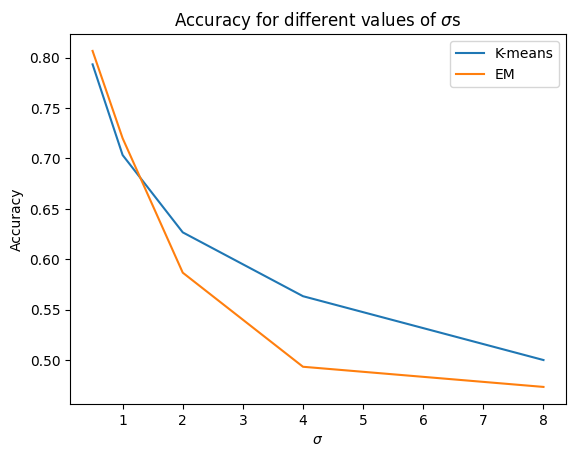
\includegraphics[scale=0.4]{Images/q12/q12_acc.png}
    \end{figure}
\end{soln}

\begin{itemize}
\item First implement K-means clustering and the expectation maximization algorithm for GMMs.
Execute both methods on five synthetic datasets,
generated as shown above with $\sigma \in \{0.5, 1, 2, 4, 8\}$. Finally, evaluate both methods on \emph{(i)} the clustering objective~\eqref{eqn:kmeans} and \emph{(ii)}  the clustering accuracy. For each of the two criteria, plot the value achieved by each method against $\sigma$.

\item Both algorithms are only guaranteed to find only a local optimum so we recommend trying multiple
restarts and picking the one with the lowest objective value (This is~\eqref{eqn:kmeans} for K-means and the negative log likelihood for GMMs).
You may also experiment with a smart initialization
strategy (such as kmeans++).

\item
To plot the clustering accuracy,  you may treat the `label' of points generated from distribution
$P_u$ as $u$, where $u\in \{a, b, c\}$.
Assume that the cluster id $i$ returned by a method is $i\in \{1, 2, 3\}$.
Since clustering is an unsupervised learning problem, you should obtain the best possible mapping
from $\{1, 2, 3\}$ to $\{a, b, c\}$ to compute the clustering objective.
One way to do this is to compare the clustering centers returned by the method (centroids for
K-means, means for GMMs) and map them to the distribution with the closest mean.

\end{itemize}

Points break down: 7 points each for implementation of each method, 6 points for reporting of
evaluation metrics.
